\documentclass[10pt]{article}
\usepackage{listings}
\usepackage{setspace}
\usepackage{multicol}
\usepackage{enumitem}
\usepackage{amsmath,amsthm,amssymb}
\usepackage{mathtools}
\usepackage{graphicx}
\usepackage{xcolor}
\usepackage{fancyhdr}
\usepackage{hyperref}

% Set margins
\usepackage[margin=2.5cm, left=1cm, right=1cm, top=1.8cm, bottom=1.8cm,headsep=0.5cm]{geometry}

% Reduce section spacing
\usepackage[compact]{titlesec}
\titlespacing{\section}{0pt}{2ex}{1ex}
\titlespacing{\subsection}{0pt}{1ex}{0ex}
\titlespacing{\subsubsection}{0pt}{0.5ex}{0ex}

% Math stuff
\DeclarePairedDelimiter{\ceil}{\lceil}{\rceil}
\DeclarePairedDelimiter\floor{\lfloor}{\rfloor}

% Image stuff
\graphicspath{ {.} }

% URL Stuff
\hypersetup{
colorlinks=true,
linkcolor=blue,
filecolor=magenta,
urlcolor=cyan,
}

% Header/Foodter setup
\pagestyle{fancy}
\fancyhf{}
\rhead{CSC413 Final Project}
\lhead{Henry Tu and Seel Patel}
\rfoot{Page \thepage}
\lfoot{April 18, 2021}

% Code style setup
\lstdefinestyle{Python}{
language = Python,
frame = lines,
numbers = left,
basicstyle = \scriptsize,
keywordstyle = \color{blue},
stringstyle = \color{green},
commentstyle = \color{red}\ttfamily
}

% To be honest, I have no idea what this is used for
\makeatletter
\renewcommand*\env@matrix[1][*\c@MaxMatrixCols c]{%
\hskip -\arraycolsep
\let\@ifnextchar\new@ifnextchar
\array{#1}}
\makeatother
\onehalfspacing

% Some not sketchy latex
\begin{document}
    \begin{center}
        \textbf{Comparing the interpretability of different GAN architectures}
    \end{center}
    \begin{minipage}{.5\textwidth}
        \centering
        \textbf{Henry Tu}\\
        University of Toronto
    \end{minipage}
    \begin{minipage}{.5\textwidth}
        \centering
        \textbf{Seel Patel}\\
        University of Toronto
    \end{minipage}
    \\
    \begin{multicols*}{2}
        \raggedcolumns

        % Document starts here
        \section{Abstract}
        \label{sec:abstract}
        A Generative Adversarial Network (GAN) uses an adversarial process between two models which are simultaneously trained to estimate a generative model.\cite{gan}
        There are many variants of GAN architectures, such as COCO-GAN\cite{cocogan} and StyleGAN\cite{stylegan}, which both have the ability to generate synthetic images which mimic real images.\\\\
        We are exploring methods of comparing the quantitative performance of these architectures with their interpretability.
        Our quantitative measures include C2ST\cite{evaluateGANs}, image quality measures\cite{evaluateGANs}, etc.\\\\
        In order to analyze these networks qualitatively, we will use methods such as Latent Space Exploration\cite{sampleGAN} and nearest neighbour tests\cite{evaluateGANs} to decipher what the networks have learned.\\\\
        By combining these two forms of analysis, we hope to gain insight into the relationship between performance metrics and the generated output of the models.

        \section{Introduction}
        \label{sec:introduction}
        StyleGAN and COCO-GAN generate images using different techniques to accomplish two different goals: StyleGAN is designed such that high level features of the output image can be finely tuned and adjusted (e.g. lighting, hair colour, etc.)\cite{stylegan}.
        On the other hand, COCO-GAN generates each part of the image separately before stitching it together in order to simulate the human perception of vision\cite{cocogan}.
        As a result, we expected each model to generate images with different qualities that relate to their designed tasks.
        \section{Dataset Generation}
        \label{sec:dataset}
        Both GAN models were trained on the LSUN Bedroom dataset\cite{lsunBedroom} at a resolution of $256 \times 256$.
        Due to time constraints, we used pre-trained models to generate images for our analysis.

        \label{sec:datasetGeneration}
        \subsection{StyleGAN}
        \label{subsec:styleganGeneration}
        NVIDIA Research Projects' Official TensorFlow Implementation of StyleGAN pretrained to the LSUN Bedroom dataset\cite{styleGANCode} was used to generate images for analysis.
        5000 latent vectors $\mathbf{z} \in \mathbb{R}^{512} \sim \mathcal{N}(0, 1\mathbf{I})$ which each correspond to an output image.

        \subsection{COCO-GAN}
        \label{subsec:cocoganGeneration}
        The TensorFlow implementation of COCO-GAN by its authors pretrained to the LSUN Bedroom dataset\cite{cocogan} was used to generate images for analysis.
        5000 latent vectors $\mathbf{z} \in [-1, 1]^{128} \sim \mathcal{U}[-1, 1]^{128}$ which each correspond to an output image. 

        \section{Quantitative Analysis}
        \label{sec:quantitative}
        \subsection{C2ST}
        \label{subsec:c2st}
        Classifier Two-Sample Tests (C2ST) is used to predict if two samples came from the same distribution\cite{c2st}.
        In the context of evaluating GANs, we will use C2ST to quantitatively measure how well the models mimic real images.
        We trained a deep convolutional neural network to perform binary classification based on the recommended discriminator architecture from \textit{Unsupervised Representation Learning
with Deep Convolutional Generative Adversarial Networks}\cite{dcgan}.
        The goal is to compare the margin by which each GAN model is able to trick the classifier to quantify image generation quality.
        \\\\
        The classifier was implemented in Pytorch with Cross Entropy loss, the Adam optimizer ($\alpha=0.1$), and the following network architecture (\# of channels per layer specified in diagram):\\
        Figure 4.1.1: \textbf{C2ST Classifier Architecture}\\
        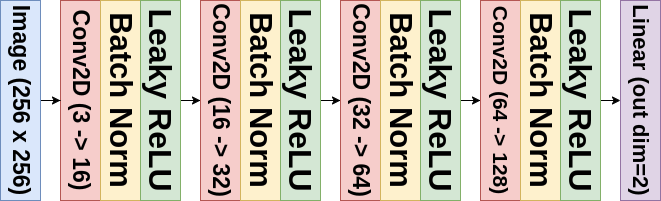
\includegraphics[scale=0.4]{c2st-diagram.png}\\
        For all Conv2D layers, \textbf{Kernel Size: 3, Stride: 2, Padding: 1, Leaky ReLU slope: 0.2}.
        Argmax is taken across output of linear units for classification.
        \\\\
        Let $\mathbf{f}: [0, 1]^{3 \times 256 \times 256} \rightarrow \mathbb{R}^{2}$ be the neural network in Figure 4.1.1. 
        Let $GANImages, RealImages \in [0, 1]^{3 \times 256 \times 256}$ be the distribution of generated images and real images respectively. For samples $\mathbf{x}_{real} \sim RealImages$ (class 1) and $\mathbf{x}_{gan} \sim GANImages$ (class 0), the predicted class $\hat{c} =argmax_c (\mathbf{f}(\mathbf{x})[c])$. The classification is correct iff $\hat{c} = class(\mathbf{x})$.
        \\
        All three datasets (training, validation, test) were drawn from $\beta RealImages + (1 - \beta)GANImages, \beta \sim Bern(0.5)$.
        Out of the combined pool of 10000 images, 5000 were allocated for training, 2500 validation, and 2500 testing.
        Let $StyleGANImages, COCOGANImages$ be the distribution of StyleGAN and COCO-GAN generated images respectively.
        \begin{center}
            Let $GANImages = \beta StyleGANImages +$\\$(1 - \beta) COCOGANImages, \beta \sim Bern(0.5)$
        \end{center}
        The model was trained with a batch size of 200 for 1000 epoches.
        After tuning hyper parameters and performing early stopping with the validation dataset, the following results were attained:\\

        \begin{tabular}{ |p{4cm}|p{3cm}|  }
         \hline
         \multicolumn{2}{|c|}{Table 1: \textbf{Real vs GAN Classifier Accuracy}} \\
         \hline
        Data Set     & Accuracy\\
         \hline
        Training        & 75.9\% of 5000 \\
         \hline
        Validation      & 67.6\% of 2500 \\
         \hline
        Test (Real)     & 58.2\% of 1250 \\
         \hline
        Test (StyleGAN) & 60.5\% of 625  \\
         \hline
        Test (COCO-GAN) & 89.6\% of 625 \\
         \hline
        \end{tabular}
        \\\\
        The model was able to correctly identify the origin of an image the majority of the time.
        This data suggests that StyleGAN is better at tricking the classifier than COCO-GAN.
        \\\\
        To confirm this, we trained additional classifiers using the same architecture, data set distribution, and hyper-parameters but only using images from one of the GAN models.
        (i.e. all 5000 generated images are all from one GAN model)
        The goal is to test how well the classifier performs when isolated to a specific GAN.
        
        Let $GANImages = StyleGANImages$\\

        \begin{tabular}{ |p{4cm}|p{4.2cm}|  }
             \hline
             \multicolumn{2}{|c|}{Table 2: \textbf{Real vs StyleGAN Classifier Accuracy}} \\
             \hline
            Data Set     & Accuracy\\
             \hline
            Training        & 77.6\% of 5000 \\
             \hline
            Validation      & 68.1\% of 2500 \\
             \hline
            Test (Real)     & 74.6\% of 1250 \\
             \hline
            Test (StyleGAN) & 61.4\% of 1250  \\
             \hline
        \end{tabular}\\
        
        Let $GANImages = COCOGANImages$\\
        
        \begin{tabular}{ |p{4cm}|p{3cm}|  }
             \hline
             \multicolumn{2}{|c|}{Table 3: \textbf{Real vs COCO-GAN Classifier Accuracy}} \\
             \hline
            Data Set     & Accuracy\\
             \hline
            Training        & 87.9\% of 5000 \\
             \hline
            Validation      & 88.2\% of 2500 \\
             \hline
            Test (Real)     & 96.4\% of 1250 \\
             \hline
            Test (COCO-GAN) & 76.1\% of 1250 \\
             \hline
        \end{tabular}
        \\
        As seen here, the Real vs COCO-GAN classifier (Table 3) performed significantly better than the Real vs StyleGAN classifier (Table 2).
        This supports the hypothesis that StyleGAN mimics real images better than COCO-GAN.
        \\\\
        Although these results suggest it is difficult for a classifier to identify a StyleGAN generated image compared to COCO-GAN, it is not a comprehensive test.
        Therefore, we must put this information in the context of the other metrics in order to draw a stronger conclusion.
        We will use SmoothGrad\cite{smoothgrad} in the Combined Analysis (Section 6.3) to qualitatively study what features of the image the classifier uses to make its decisions.

        \subsection{Image Sharpness}
        \label{subsec:imageSharpness}
        A common indicator of image quality is sharpness.
        When an image is sharp, the details within the image are seen more clearly and there is a better distinction between different objects in the picture.
        Overall, this allows humans to form a better understanding of what they are seeing when they view the image.
        Using directional image gradients along the $x$ and $y$ axes, we measured the mean image sharpness of the generated images and real images as seen below. (Higher is better)\\

        %%%%%%%%%%%%%%%%%%%%%%%%%%
        % Comment: Should also mention how many images were used in this analysis
        \begin{tabular}{ |p{2cm}|p{2cm}|p{2cm}|p{2cm}|  }
             \hline
             \multicolumn{4}{|c|}{Table 4: \textbf{Mean Image Sharpness}} \\
             \hline
            & Real & StyleGAN & COCO-GAN  \\
            \hline
            Sharpness & 8.534    & 8.214      & 7.970\\
            \hline
        \end{tabular}
        \\\\
        Therefore the real images are the sharpest and StyleGAN does the better job of producing sharper images than COCO-GAN.
        However, does higher sharpness always mean better image quality?
        We explore this question in the combined analysis section below.

        \subsection{Color Distribution Comparison}
        \label{subsec:colorDistribution}
        The purpose of a GAN is to generate new images that match the distribution of the training images. Therefore, we decided to statistically compare the distribution of generated images with the distribution of real images in order to understand how well the GANs have fit to the training data.
        \\\\
        In order to properly mimic the real images, the generated images have to closely follow the color distribution of the real images. Each image in our data is represented by RGB values ranging between 0 and 1. We extracted the frequencies of RGB color values using 25 bins for each of the datasets. The distribution of these frequencies are plotted below for the real images and each set of generated data.
        \\
        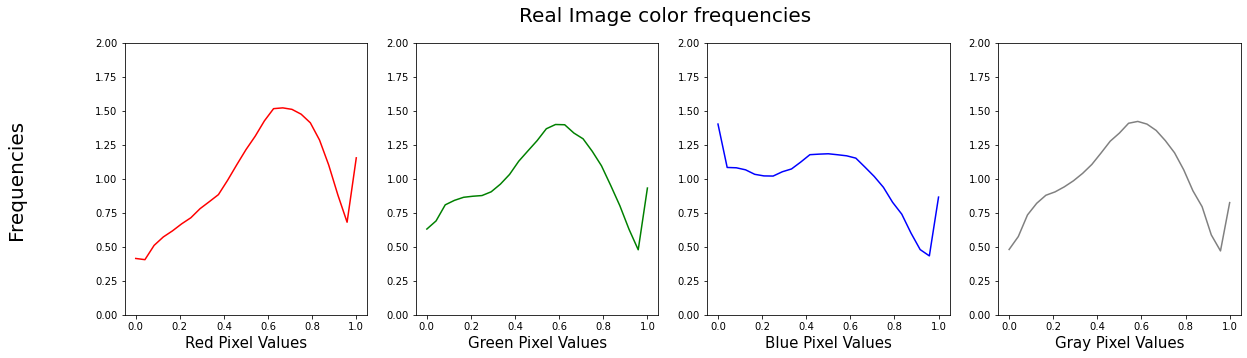
\includegraphics[scale =0.21]{color-distributions/real_color_freq.png}
        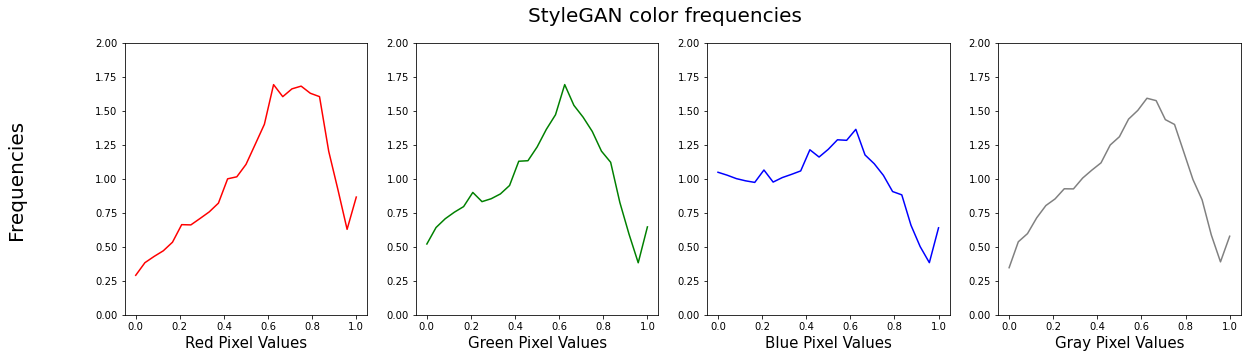
\includegraphics[scale =0.21]{color-distributions/stylegan_color_freq.png}
        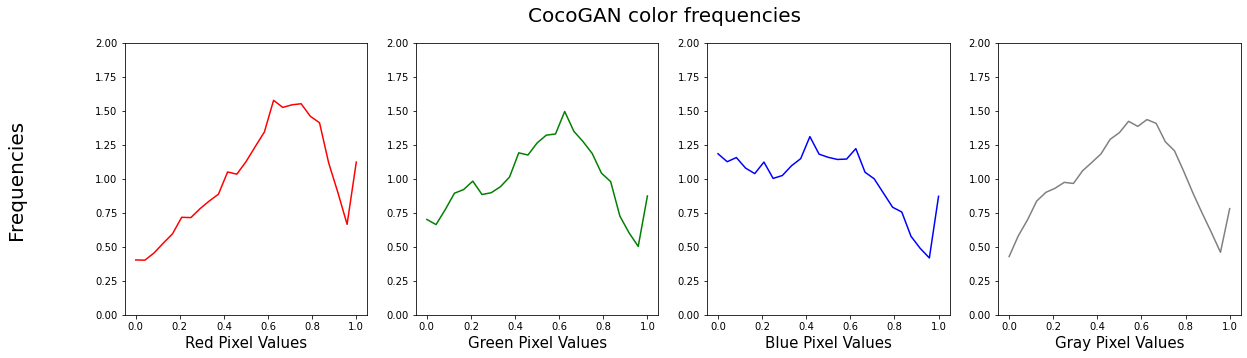
\includegraphics[scale =0.21]{color-distributions/cocogan_color_freq.png}
        \\
        As seen in the frequency plots, both StyleGAN and COCO-GAN do a good job of modelling the real distribution of colors.
        However, both generated image frequency plots show many spikes that are not present in the real image frequency plots.
        We will explore these spikes in our combined analysis section. Additionally, to quantify this color reproduction quality, we also took the KL Divergence between the color distributions of each model to the real images.\\\\
        %%%%%%%%%%%%%%%%%%%%%%%%%%
        % Comment: Should also mention how many images were used in this analysis
        \begin{tabular}{ |p{2cm}|p{1cm}|p{1cm}|p{1cm}|p{1cm}|  }
             \hline
             \multicolumn{5}{|c|}{Table 5: \textbf{KL divergence of color channels w/ real imgs}} \\
             \hline
            & Red & Green & Blue & Gray  \\
            \hline
            StyleGAN & 0.286    & 0.263      & 0.232     &  0.251 \\
            \hline
            COCO-GAN  & 0.044    & 0.047      & 0.059     &  0.016\\
            \hline
        \end{tabular}
        \\\\
        Therefore COCO-GAN does a statistically better job of modelling the color distribution of the real images. Note that this does not guarantee that COCO-GAN is superior because this method of comparison does not take into account the spatial position of the colors. This means that the images would post the same KL Divergence even if the pixels were scrambled. Therefore further analysis is needed to determine which model performs better overall.


        \section{Qualitative Analysis}
        \label{sec:qualitative}
        \subsection{Latent Space Exploration}
        \label{subsec:latentSpaceExploration}
        An important part of the generator is it's ability to combine different features from the real image in order to generate new images.
        For example, in our dataset, an image could contain a bed, a window or a painting. What about a combination of these?
        What if the locations of these features is changed? We use latent space interpolation to determine if the model produces robust images in all of these cases.

        \subsection{Nearest Neighbours}
        \label{subsec:nearestneighbours}
        A common problem within GANs is mode collapse.
        This occurs when the generator consistently outputs the same image for distinct latent vectors.
        In addition to this, we want to identify if the generator creates multiple images with identical structure or color scheme.
        To identify these issues, we randomly sampled generated images and visually compared them with the k nearest neighbours from the images produced by the same model.
        In our search, we found no evidence of mode collapse in either StyleGAN or COCO-GAN. Samples from the images used in this analysis are provided below.

        \section{Combined Analysis}
        \label{sec:combinedAnalysis}
        \subsection{Colour Frequency Peaks}
        In our analysis of color frequency distributions above, we noticed that both StyleGAN and COCO-GAN exhibited spikes in their frequency graphs.
        One prominent spike occurs simultaneously in the green and blue channel at intensity level 0.6.
        This occurs in both the StyleGAN and COCO-GAN generated images.
        Specifically, this spike happened in colors covered by the following gradient.\\
        Figure 6.1.1: \textbf{(0,0.6,0.6)$\longrightarrow$(1.0,0.6,0.6) RGB Gradient} \\
        
\includegraphics[scale=0.1]{gradient.png} \\
        We decided to sample some of these colors and found generated images with color schemes closely matching them.
        The images matching color $(0.3, 0.6, 0.6)$ can be seen below for both StyleGAN and COCO-GAN. \\
        Figure 6.1.2: \textbf{COCO-GAN Images} \\
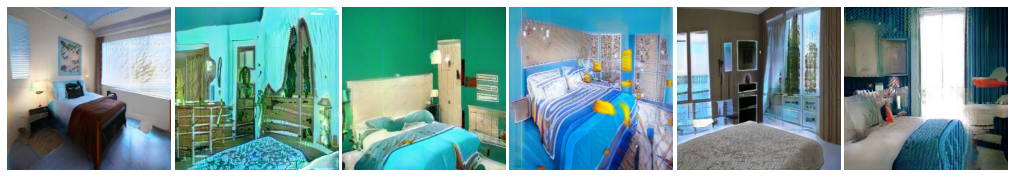
\includegraphics[scale=0.28]{color-images/03_06_06_coco_images.png} \\
        Figure 6.1.3: \textbf{StyleGAN Images} \\
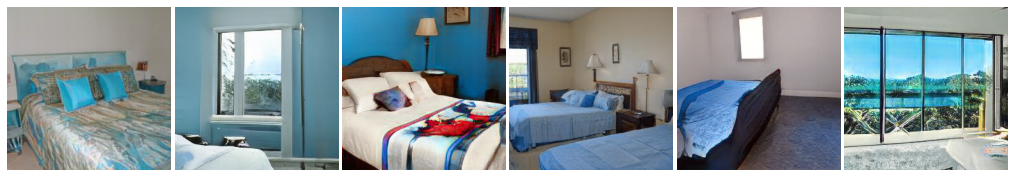
\includegraphics[scale=0.28]{color-images/03_06_06_stylegan_images.png} \\
        For both models, we are seeing an increase in noise and distortion in the images.
        This is especially true in the case of COCO-GAN, for which every image displays noisy textures or bad structure.
        What does this trend tell us about COCO-GAN?
        From the samples, we can see that many of these images have windows in them that display the sky.
        COCO-GAN has done a relatively poor job of displaying the sky and natural imagery in the background.
        \\\\
        Additionally in the COCO-GAN images we can see that much of the color from the sky bleeds into other parts of the image.
        These sky colors are very similar to the colors in the gradient we are studying.
        Therefore we theorize that this spike in frequency occurs from COCO-GAN being unable to properly generate images that include the sky.
        %
        %
        %
        %
        %
        \subsection{High Sharpness Images}
        In our analysis of image sharpness, we found that StyleGAN produced sharper images than COCO-GAN.
        In order to qualitatively explore what higher sharpness means, we have plotted the sharpest images produced by both models.\\
        
        Figure 6.2.1: \textbf{Sharpest COCO-GAN Images} \\
        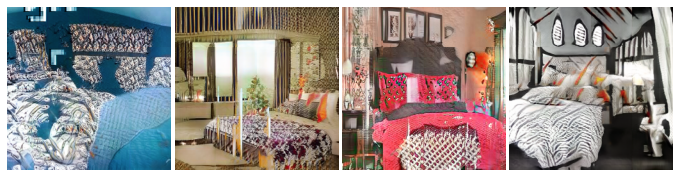
\includegraphics[scale=0.35]{sharpness-images/coco_sharpness.png}
        \\ Figure 6.2.2: \textbf{Sharpest StyleGAN Images}\\
        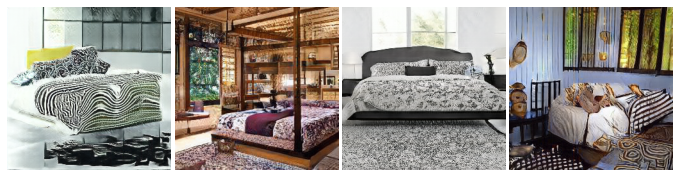
\includegraphics[scale=0.35]{sharpness-images/stylegan_sharpness.png}
        \\
        As we can see, the StyleGAN images are of high quality, but the COCO-GAN images are consistently filled with noisy patterns.
        Both sets consist of very sharp images, and therefore we have visualized the sharpness below in order to understand why there is such a large difference in quality.
        \\ Figure 6.2.3: \textbf{COCO-GAN Sharpness Visualization}\\
        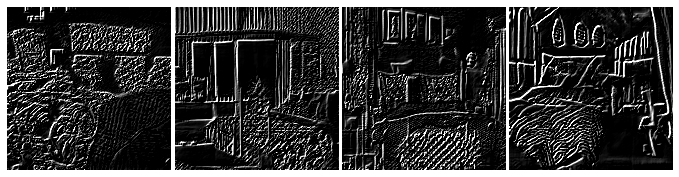
\includegraphics[scale=0.35]{sharpness-images/coco_sharpness_lines.png}
        \\ Figure 6.2.4: \textbf{StyleGAN Sharpness Visualization}\\
        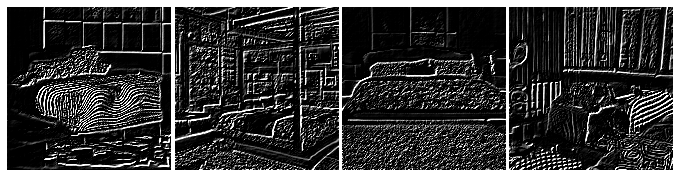
\includegraphics[scale=0.35]{sharpness-images/stylegan_sharpness_lines.png}
        \\
        By comparing the sharpness plots to the images, we can see that the sharpness of the StyleGAN images comes from it's ability to effectively generate complex patterns.
        However, the sharpness of the COCO-GAN images comes from unwanted noise or messy patterns which are often out of place.
        Therefore, even though both models produce images with a relatively similar sharpness, the sharper images produced by StyleGAN are vastly superior to those produced by COCO-GAN.
        In conclusion, the qualitative results indicate that the true quality of COCO-GAN images may be lower than the numbers indicate.
        
        \subsection{C2ST Smoothgrad Analysis}
        Now that we've quantitatively showed that images generated by StyleGAN are difficult to distinguish from real images than COCO-GAN, we can use SmoothGrad to generate a sensitivity map to visually discover which parts of the image most strongly affects the classification \cite{smoothgrad}.
        \\\\
        Smoothgrad was performed on all 3 classifier models outlined in the C2ST section from earlier. 
        Let $\mathbf{x} \in [0, 1]^{3 \times 256 \times 256}$ be the input image, $\mathcal{L}$ be CE loss, and $\nabla_{\mathbf{x}}^{*} \mathcal{L} (\mathbf{x})$ be the sensitivity map.
        \begin{center}
            $\nabla_{\mathbf{x}}^{*} \mathcal{L} (\mathbf{x}) = \frac{1}{100} \sum_{i=1}^{100} \nabla_{\mathbf{x}} \mathcal{L} (\mathbf{x} + \mathcal{N}(0, 0.1^2\mathbf{I})) $
        \end{center}
        The following is a selection of sensitivity maps of correct classifications: (Full samples available in Appendix 6.3.*)\\ 
        Figure 6.3.1: \textbf{Real vs GAN Classifier Sensitivity}
        \begin{verbatim}Real Image    StyleGAN Img COCO-GAN Img\end{verbatim}
        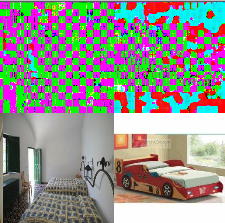
\includegraphics[scale=0.3]{smoothgrad/combined/real.png}
        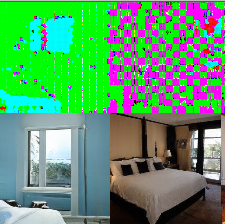
\includegraphics[scale=0.3]{smoothgrad/combined/stylegan.png}
        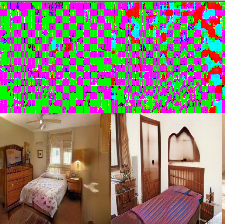
\includegraphics[scale=0.3]{smoothgrad/combined/coco.png}\\
        Evidently, there is a clear checkerboard pattern, which could be caused by COCO-GAN's tile generation\cite{cocogan}. 
        We can use the classifier trained on only one GAN to validate this theory.\\
        Fig 6.3.2: \textbf{Real vs StyleGAN Classifier Sensitivity}
        \begin{verbatim}Real Image    StyleGAN Image\end{verbatim}
        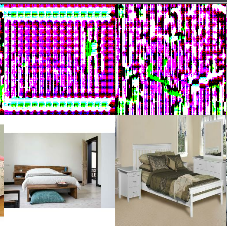
\includegraphics[scale=0.3]{smoothgrad/stylegan/real.png}
        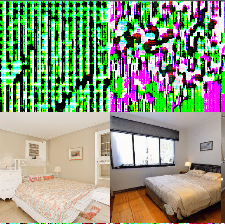
\includegraphics[scale=0.3]{smoothgrad/stylegan/stylegan.png}\\
        Fig 6.3.3: \textbf{Real vs COCO-GAN Classifier Sensitivity}
        \begin{verbatim}Real Image    COCO-GAN Image\end{verbatim}
        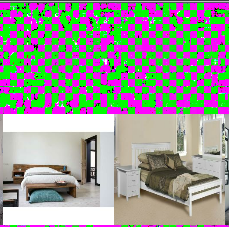
\includegraphics[scale=0.3]{smoothgrad/coco/real.png}
        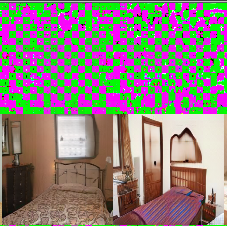
\includegraphics[scale=0.3]{smoothgrad/coco/coco.png}\\
        As seen in Fig 6.3.3, the Real vs COCO-GAN classifier uses a checkerboard filter, which is quite effective with a test accuracy of $\frac{76.1\% + 96.4\%}{2} = 86.3\%$ (Table 3). 
        On the other hand, the StyleGAN classifier (Fig 6.3.2) is very uniform and shows very few artifacts.
        This seems to suggest there are irregularities in between tiles generated by COCO-GAN which are easily detected by the classifier.
        Therefore according to C2ST, StyleGAN produces more realistic images than COCO-GAN.
    \end{multicols*}
    \newpage
    \begin{thebibliography}{9}
        \bibitem{gan}
        Ian J. Goodfellow, Jean Pouget-Abadie, Mehdi Mirza, Bing Xu, David Warde-Farley, Sherjil Ozair, Aaron Courville, and Yoshua Bengio. (2014)
        \href{https://papers.nips.cc/paper/2014/file/5ca3e9b122f61f8f06494c97b1afccf3-Paper.pdf}{\textit{Generative Adversarial Networks} }

        \bibitem{cocogan}
        Chieh Hubert Lin, Chia-Che Chang, Yu-Sheng Chen, Da-Cheng Juan, Wei Wei, Hwann-Tzong Chen. (2019)
        \href{https://arxiv.org/pdf/1904.00284.pdf}{\textit{COCO-GAN: Generation by Parts via Conditional Coordinating} }

        \bibitem{stylegan}
        Tero Karras, Samuli Laine, Timo Aila. (2018)
        \href{https://arxiv.org/pdf/1812.04948.pdf}{\textit{A Style-Based Generator Architecture for Generative Adversarial Networks} }

        \bibitem{evaluateGANs}
        Brownlee, Jason. (2019)
        \href{https://machinelearningmastery.com/how-to-evaluate-generative-adversarial-networks/}{\textit{How to

        \bibitem{sampleGAN}
        Tom White. (2016)
        \href{https://arxiv.org/pdf/1609.04468.pdf}{\textit{Sampling Generative Networks} }

        \bibitem{lsunBedroom}
        Yu, Fisher and Zhang, Yinda and Song, Shuran and Seff, Ari and Xiao, Jianxiong. (2015)
        \href{https://arxiv.org/pdf/1506.03365.pdf}{\textit{LSUN: Construction of a Large-scale Image Dataset using Deep Learning with Humans in the Loop}}

        \bibitem{styleGANCode}
        NVLabs. (2019) \href{https://github.com/NVlabs/stylegan}{\textit{StyleGAN — Official TensorFlow Implementation}}

        \bibitem{c2st}
        David Lopez-Paz, Maxime Oquab. (2016)
        \href{https://research.fb.com/wp-content/uploads/2017/04/neural_tests.pdf?}{\textit{Revisiting Classifier Two-Sample Tests for GAN Evaluation and Causal Discovery}}

        \bibitem{dcgan}
        Alec Radford, Luke Metz, Soumith Chintala. (2015)
        \href{https://arxiv.org/pdf/1511.06434.pdf}{\textit{Unsupervised Representation Learning with Deep Convolutional Generative Adversarial Networks}}

        \bibitem{smoothgrad}
        Daniel Smilko, Nikhil Thorat, Been Kim, Fernanda Viegas, Martin Wattenberg (2017)
        \href{https://arxiv.org/pdf/1706.03825.pdf}{SmoothGrad: removing noise by adding noise}

    \end{thebibliography}

    \newpage
    \section{Appendix}
    Appendix 6.3.1: \textbf{Real vs GAN Classifier Sensitivity - Real Image}\\
    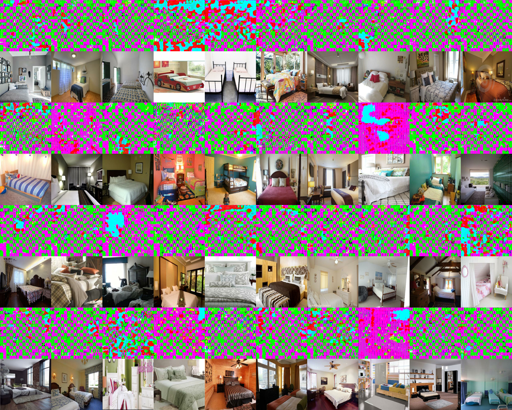
\includegraphics[scale=1.05]{smoothgrad-big/combined_model/testing-3-2-combined-dataset-raw-smoothgrad.png}\\
    Appendix 6.3.2: \textbf{Real vs GAN Classifier Sensitivity - StyleGAN}\\
    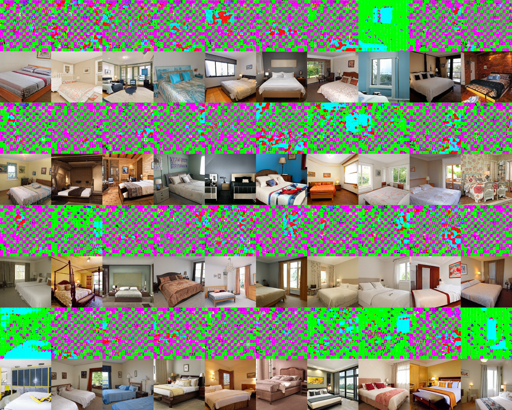
\includegraphics[scale=1.05]{smoothgrad-big/combined_model/testing-3-2-combined-dataset-stylegan-smoothgrad.png}
    \newpage
    Appendix 6.3.3: \textbf{Real vs GAN Classifier Sensitivity - COCO-GAN}\\
    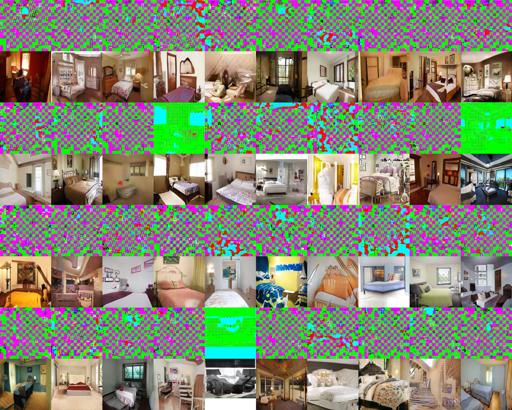
\includegraphics[scale=1.05]{smoothgrad-big/combined_model/testing-3-2-combined-dataset-coco-smoothgrad.png}\\
    Appendix 6.3.4: \textbf{Real vs StyleGAN Classifier Sensitivity - Real Image}\\
    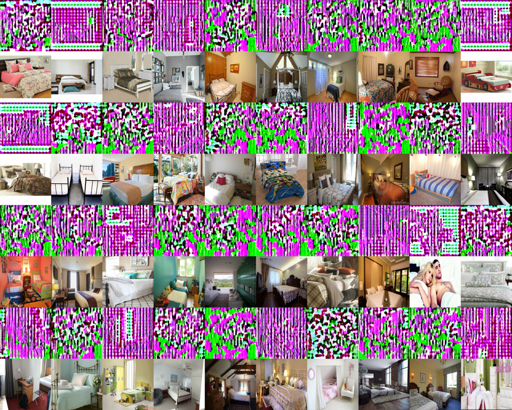
\includegraphics[scale=1.05]{smoothgrad-big/stylegan_model/testing-2-2-combined-dataset-raw-smoothgrad.png}
    \newpage
    Appendix 6.3.5: \textbf{Real vs StyleGAN Classifier Sensitivity - StyleGAN}\\
    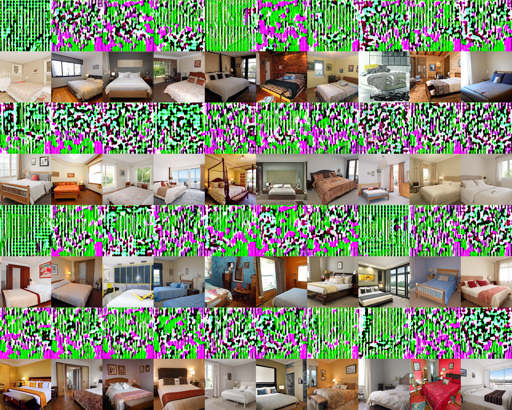
\includegraphics[scale=1.05]{smoothgrad-big/stylegan_model/testing-2-2-combined-dataset-stylegan-smoothgrad.png}\\
    Appendix 6.3.6: \textbf{Real vs COCO-GAN Classifier Sensitivity - Real Image}\\
    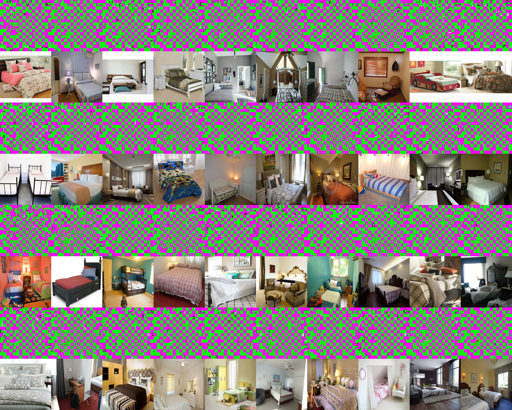
\includegraphics[scale=1.05]{smoothgrad-big/cocogan_model/testing-2-2-combined-dataset-raw-smoothgrad.png}
    \newpage
    Appendix 6.3.7: \textbf{Real vs COCO-GAN Classifier Sensitivity - COCO-GAN}\\
    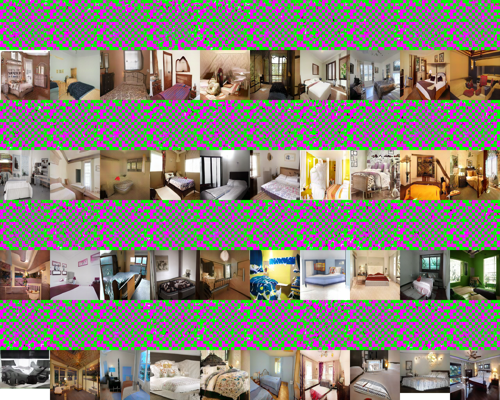
\includegraphics[scale=1.05]{smoothgrad-big/cocogan_model/testing-2-2-combined-dataset-cocogan-smoothgrad.png}

\end{document}